\documentclass[dvipdfmx,tikz]{standalone}
\usepackage{tikz}
\usepackage{ifthen}

\usetikzlibrary{
  shapes,
  shapes.geometric,
  arrows.meta,
  calc,
}

\definecolor{c0}{rgb}{0.00,0.00,0.50}
\definecolor{c1}{rgb}{0.00,0.00,1.00}
\definecolor{c2}{rgb}{0.00,0.39,1.00}
\definecolor{c3}{rgb}{0.00,0.83,1.00}
\definecolor{c4}{rgb}{0.30,1.00,0.66}
\definecolor{c5}{rgb}{0.66,1.00,0.30}
\definecolor{c6}{rgb}{1.00,0.90,0.00}
\definecolor{c7}{rgb}{1.00,0.49,0.00}
\definecolor{c8}{rgb}{1.00,0.08,0.00}
\definecolor{c9}{rgb}{0.50,0.00,0.00}


\begin{document}
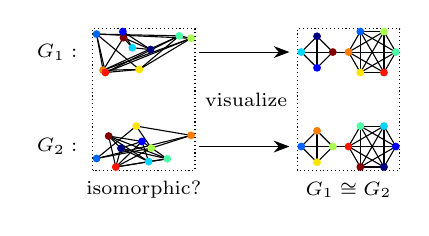
\begin{tikzpicture}
  \node at (-2.3,+0.6) {\scriptsize{$G_1:$}};
  \node at (-2.3,-0.6) {\scriptsize{$G_2:$}};
  \node at (-1.2,-1.15) {\scriptsize{isomorphic?}};
  \node at (+1.4,-1.15) {\scriptsize{$G_1 \cong G_2$}};
  \node[anchor=center] at (0.1,0) {\scriptsize{visualize}};
  \draw[-{Stealth[length=2mm]}] (-0.5,+0.6) -- (+0.65,+0.6);
  \draw[-{Stealth[length=2mm]}] (-0.5,-0.6) -- (+0.65,-0.6);
  \draw[densely dotted] (-1.85,-0.9) rectangle (-0.55,0.9);
  \draw[densely dotted] (+0.75,-0.9) rectangle (+2.05,0.9);

  \foreach \xa/\ya/\xb/\yb/\xc/\yc/\xd/\yd/\xe/\ye/\xf/\yf/\xg/\yg/\xh/\yh/\xi/\yi/\xj/\yj/\xS/\yS/\ord in {
      -0.158/0.183/0.186/0.032/-0.046/0.055/-0.166/0.260/-0.417/-0.231/0.043/-0.221/-0.388/-0.260/0.551/0.206/0.700/0.175/-0.500/0.228/-1.3/+0.6/0,
      0.195/-0.020/0.700/0.142/-0.500/-0.152/0.004/0.260/-0.256/-0.260/-0.346/0.133/-0.190/-0.022/0.076/0.065/0.161/-0.191/0.398/-0.156/-1.3/-0.6/1,
      -0.100/0.000/-0.300/0.200/-0.500/0.000/-0.300/-0.200/0.100/0.000/0.250/-0.260/0.550/-0.260/0.700/-0.000/0.550/0.260/0.250/0.260/+1.3/+0.6/0,
      -0.100/0.000/-0.300/0.200/-0.500/0.000/-0.300/-0.200/0.100/0.000/0.250/-0.260/0.550/-0.260/0.700/-0.000/0.550/0.260/0.250/0.260/+1.3/-0.6/1
    }{
      \begin{scope}[shift={{(\xS,\yS)}}]
        \coordinate (a) at (\xa,\ya);
        \coordinate (b) at (\xb,\yb);
        \coordinate (c) at (\xc,\yc);
        \coordinate (d) at (\xd,\yd);
        \coordinate (e) at (\xe,\ye);
        \coordinate (f) at (\xf,\yf);
        \coordinate (g) at (\xg,\yg);
        \coordinate (h) at (\xh,\yh);
        \coordinate (i) at (\xi,\yi);
        \coordinate (j) at (\xj,\yj);
        \draw (a) -- (e);
        \draw (a) -- (b);
        \draw (a) -- (c);
        \draw (a) -- (d);
        \draw (b) -- (c);
        \draw (b) -- (d);
        \draw (c) -- (d);
        \draw (e) -- (f);
        \draw (e) -- (g);
        \draw (e) -- (h);
        \draw (e) -- (i);
        \draw (e) -- (j);
        \draw (f) -- (g);
        \draw (f) -- (h);
        \draw (f) -- (i);
        \draw (f) -- (j);
        \draw (g) -- (h);
        \draw (g) -- (i);
        \draw (g) -- (j);
        \draw (h) -- (i);
        \draw (h) -- (j);
        \draw (i) -- (j);
        \ifthenelse{\ord=0}{
          \node[draw=none,circle,inner sep=1pt,fill=c9] at (a) {};
          \node[draw=none,circle,inner sep=1pt,fill=c0] at (b) {};
          \node[draw=none,circle,inner sep=1pt,fill=c3] at (c) {};
          \node[draw=none,circle,inner sep=1pt,fill=c1] at (d) {};
          \node[draw=none,circle,inner sep=1pt,fill=c7] at (e) {};
          \node[draw=none,circle,inner sep=1pt,fill=c6] at (f) {};
          \node[draw=none,circle,inner sep=1pt,fill=c8] at (g) {};
          \node[draw=none,circle,inner sep=1pt,fill=c4] at (h) {};
          \node[draw=none,circle,inner sep=1pt,fill=c5] at (i) {};
          \node[draw=none,circle,inner sep=1pt,fill=c2] at (j) {};
        }{
          \node[draw=none,circle,inner sep=1pt,fill=c5] at (a) {};
          \node[draw=none,circle,inner sep=1pt,fill=c7] at (b) {};
          \node[draw=none,circle,inner sep=1pt,fill=c2] at (c) {};
          \node[draw=none,circle,inner sep=1pt,fill=c6] at (d) {};
          \node[draw=none,circle,inner sep=1pt,fill=c8] at (e) {};
          \node[draw=none,circle,inner sep=1pt,fill=c9] at (f) {};
          \node[draw=none,circle,inner sep=1pt,fill=c0] at (g) {};
          \node[draw=none,circle,inner sep=1pt,fill=c1] at (h) {};
          \node[draw=none,circle,inner sep=1pt,fill=c3] at (i) {};
          \node[draw=none,circle,inner sep=1pt,fill=c4] at (j) {};
        }
      \end{scope}
    }
\end{tikzpicture}
\end{document}